\documentclass[10pt]{article}

\usepackage{amsmath}                                                                % Math mode $-$ o $$-$$
\usepackage{amssymb}                                                                % Mathematic symbols
\usepackage{mathrsfs}                                                               % Caligraphic letters
\usepackage{amsthm}                                                                 % Theorem-like environments

\usepackage[english]{babel}                                                         % Language (it is important when hyphenating words)
\usepackage[utf8]{inputenc}                                                         % Accented letters and other strange symbols

\usepackage{graphicx}                                                               % Images
\usepackage{float}                                                                  % Puts images where they belong
\usepackage{subcaption}                                                             % Subimages
\usepackage{wrapfig}                                                                % Text and image on the same line
\usepackage{subfiles}                                                               % Subfiles
\usepackage[hidelinks]{hyperref}                                                    % Allows external and internal references
\usepackage[nameinlink]{cleveref}                                                   % Improves internal references
\usepackage[super,square]{natbib}                                                   % Easy bibliography

\usepackage{verbatim}                                                               % Verbatim + multiline comments
\usepackage{anysize}\marginsize{2cm}{2cm}{.5cm}{3cm}                                % Personalizes margins: {L}{R}{U}{D}
\usepackage{bbm}                                                                    % Allows \1
\usepackage{mathdots}                                                               % Rising triple dot symbol
\usepackage{faktor}                                                                 % Fancy rendering of coset sets
\usepackage{tikz-cd}                                                                % Commutative diagrams
\usetikzlibrary{babel}                                                              % Avoids interference between tikz-cd i babel
\usepackage{lipsum}                                                                 % Lorem ipsum dolor sit amet, with \lipsum or \lipsum[1]
\usepackage{todonotes}                                                              % To indicate something is missing
\usepackage[normalem]{ulem}
\usepackage{graphicx}

\usepackage{amsthm}
\usepackage{xcolor}
\usepackage{tcolorbox}
\newtcbox{\mybox}{on line,
  colframe=blue,colback=blue!10!white,
  boxrule=0.5pt,arc=4pt,boxsep=0pt,left=6pt,right=6pt,top=6pt,bottom=6pt}
\usepackage{float}
\usepackage{hyperref}
\hypersetup{
    colorlinks = true,
    filecolor = blue,
    linkcolor = blue,
    urlcolor = blue,
}

\thispagestyle{empty}

\begin{document}
\begingroup
  \centering
  \Huge Wine type and quality determination \\
  \vskip 0.35cm
  \LARGE Final delivery\\
  \vskip 0.25cm
  \large Aleix Torres i Camps, Àlex Batlle Casellas, Luís Sierra Muntané\\[1.5em]
\endgroup


\section{Description and goals of the project.}
Our goal with this project is that of obtaining a data-driven understanding of the relationships between the chemical characteristics of wine and features such as its colour or quality. The data in question is \href{http://archive.ics.uci.edu/ml/datasets/Wine+Quality}{this data set} featuring Portuguese wines of the \textit{Vinho Verde} region and claims to have 4898 instances of wines, even though after looking at the dataset we saw there actually were 6497, and 12 attributes as physicochemical properties of the wine: \verb|fixed acidity|, \verb|volatile acidity|, \verb|citric acid|, \verb|residual sugar|, \verb|chlorides|, \verb|free sulfur dioxide|, \verb|total sulfur dioxide|, \verb|density|, \verb|pH|, \verb|sulphates|, \verb|alcohol|, and \verb|quality| (score between 0 and 10) which is the output variable based on sensory data.
Furthermore, we consider whether the wine is red or white, given that there are two datasets, one for each colour of wine. \\

As such, the \textbf{main objective} will be that of classifying the wines into their corresponding colour class as white or red from their physicochemical properties, but also to determine their quality on a scale of 0 to 10 as subjectively decided by a panel of experts from their sensory perceptions of the wine. As such, we will want to see whether there are variables which can strongly predict the final quality of a wine or whether such variables are even relevant in determining such a metric. This is especially relevant since the variables, which are all real numbers, are usually associated with being important qualities for the wine and its final taste. All in all, the variable representing the colour of the wine will be predicted from the 11 explanatory variables and the variable representing the quality of the wine will be predicted using the 11 explanatory variables and the colour of the wine as well. It remains to be seen whether they will be good to predict the final factor variables of colour and quality, and to discern which variables yield better models for the prediction of the target variables.

\section{Related previous work.}
This data set has been previously used in various projects, as wine appears to be a frequent topic in examples of classification problems in ML. The first one we cite here is the one provided as a relevant paper, \href{https://www.sciencedirect.com/science/article/pii/S0167923609001377?via\%3Dihub}{Modeling wine preferences by data mining from physicochemical properties}. This paper, as it states in its abstract, proposes a data mining approach to predict human taste preferences on wine, through three different types of regression model: multiple regression, neural networks and support vector machines. This goal is similar to ours, but uses models we cannot comment on for the moment, as they have not been explained in class yet. \\

Apart from the data set webpage, we have looked for other projects that cite and use this data set. Searching through Kaggle we have found some different kernels operating on this data. Some of these use decision tree-based methods and support vector machines so we are not commenting on them either. Even though, they also use linear and generalized linear models to preliminary test variable significance. \\

The \href{https://www.kaggle.com/indra90/predicting-white-wine-quality}{first kernel} only uses white wine data. One thing to remark about most of the models used on this kernel is that they binarize the quality of the wines into "good" and "not good" and then use the previous stated models and logistic regression. \\

In the \href{https://www.kaggle.com/conradws/how-good-is-this-wine-m-l-for-quality-control}{second kernel}, it is remarkable the various ways in which the author tries to gain insight on the data. Initially they use k-Means to cluster data, and then based on the results of this method they visualize the data using a Radial Visualization (RadViz) plot, which we can map into our knowledge as being similar to a biplot. In this way they can observe if there exist any clear tendencies as to variable influence in wine quality. They also pay special attention to anomalies throughout the notebook. \\

The \href{https://www.kaggle.com/danielpanizzo/red-and-white-wine-quality}{third kernel} we are commenting on is an exploratory data analysis into the data. In this work it is remarkable the univariate distribution exploration, and especially the fact that this is done separately with white and red wine. This indicates that these two variants might need different treatment, which makes our second task (classification into red or white wine) pertinent in the combined data set. \\

We found some additional data exploration notebooks: namely, \href{https://rstudio-pubs-static.s3.amazonaws.com/57835_c4ace81da9dc45438ad0c286bcbb4224.html}{this one} performs some comparative plots between variables and their correlations, and \href{http://rstudio-pubs-static.s3.amazonaws.com/219996_9cc8cf9f2e7e41fe8912454c3ad2685a.html}{this other one} also investigates univariate, bivariate and multivariate relationships between variables.
\section{Data exploration.}
First of all, the data set is given into two different tables, one for red and the other for white wine. Then we decided to perform the union and \textbf{obtain an unique data set}. After that, we extracted the two target vectors. The first one, \textit{wine.type}, determines if the wine is red or white and the second one, \textit{wine.quality}, is the quality value given by the oenologist. \\

After some exploration, we detected something that we did not expect: some rows have the exact same values in all of the variables, so we concluded that there are \textbf{duplicated rows} in the data set. So we went back and decided to delete the duplicated ones and leave just one of them. But a major problem was found, 2 rows were at the same time in the two original data sets. In this situation we decided, for now, to delete the rows from both tables, as we do not know whether they belong to red or to white wines, and we still have a lot of other rows. \\

Now, we were interested in the \textbf{dimensions of the data set}. So we observed there are 5318 rows and 11 input variables. From these rows, 1357 are red wines and 3959 white. And the table of wine quality with respect to the numbers of rows with that value is:
\begin{table}[H]
\caption{Number of wines of each quality}
\centering
\begin{tabular}{|c|c|c|c|c|c|c|c|}
\hline
wine quality  & 3  & 4   & 5    & 6    & 7    & 8   & 9 \\ \hline
num. of wines & 30 & 206 & 1751 & 2323 & 855  & 148 & 5 \\ \hline
\end{tabular}
\end{table}
\ \\
Then, from these information we may extract some conclusions. The first one is that not all possible marks ([0,10]) were given. And more important, \textbf{the data set is unbalanced} with respect to wine type and wine quality. There are three times white wines as red ones and most of the marks are 6's or 5's, followed by 7's, while the other ones have a very small amount. \\

The next thing we did is caring about \textbf{missing values}. After some exploration using \textit{summary} and some \textit{histograms}, the conclusion is that there are no missing values. Although a variable was suspicious, \textit{citric.acid}, because it has a very large amount of 0 values, most of them coming from the white wines. We investigated a little bit on the topic and found that it is a supplement used as a natural preservative or a flavour potential, so we may assume that some wines have no citric acid at all. \\

In the review of the data, some \textbf{outliers} were found. Such as some wine with 1.66 in \textit{citric.acid}, while the 3rd quartile of this variable is 0.4, or another with \textit{residual.sugar} 65.8, while its 3rd quartile is 7.5. For the moment we decided to keep them but we may delete them in the future. \\

So then, we perform a \textbf{particular analysis of each variable}. We saw that all the variables of the new data set are numerical, therefore we can perform computations over them. But two variables seem to be discrete (\textit{free.sulfur.dioxide} and \textit{total.sulfur.dioxide}). One of the target variables is also discrete and the other is a factor of two elements.\\

We start by plotting the \textbf{histograms}, with different colors for each wine type. We detect that for \textit{fixed.acidity}, \textit{volatile.acidity} and \textit{citric.acid}, the two wine types have different behaviours: the white type is more like a normal distribution, while the red is flatter and in some cases looks more like a uniform distribution. These variables have in common that all of them are related to acidity so maybe in the future we might join them and create a unique variable.
\begin{figure}[H]
\centering
\caption{Histograms of 3 variables}
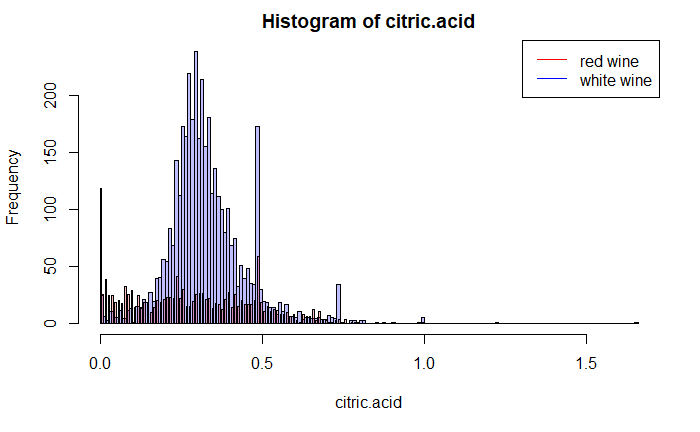
\includegraphics[scale=0.3]{histogram_of_citricacidity}
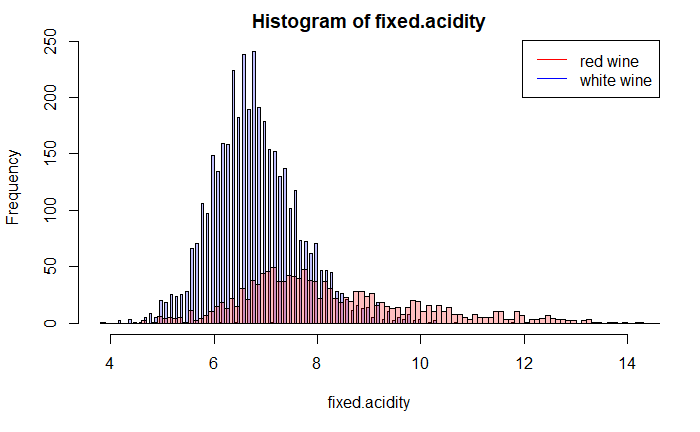
\includegraphics[scale=0.3]{histogram_of_fixedacidity}
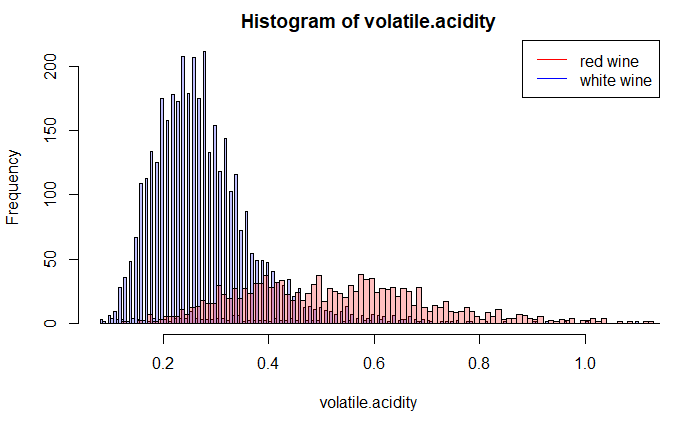
\includegraphics[scale=0.3]{histogram_of_volatileacidity}
\end{figure}
The second thing we detected is that the variable \textit{residual.sugar} has a lot of small entries, so we considered applying a logarithm and seeing the result. There is a clear improvement, and something interesting was discovered. The red wine can be modeled as a unique normal distribution while the white wine as two of them, as there are two density regions with a separation between them. So we can treat the logarithm of the \textit{residual.sugar} as a useful \textbf{feature}.
\begin{figure}[H]
\centering
\caption{Histograms of \textit{residual.sugar} and its logarithm}
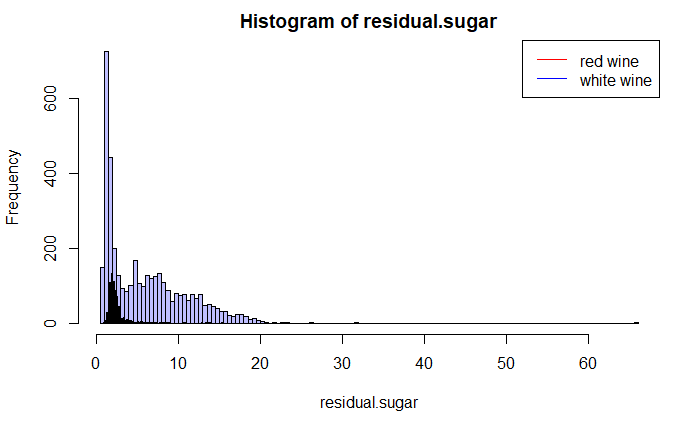
\includegraphics[scale=0.4]{histogram_of_residualsugar}
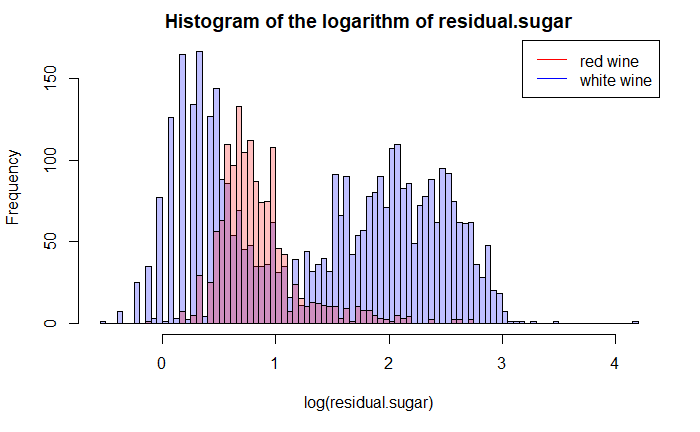
\includegraphics[scale=0.4]{histogram_of_log_residualsugar}
\end{figure}
Finally, the other variables \textit{histograms} have a \textbf{similar shape} in both wine types, but usually with \textbf{different means}. This fact could be useful in order to perform \textit{classification}. And it will be relevant as well for the \textit{regression model} to differentiate the \textit{wine.type} as factors. Here are some of the other \textit{histograms}:
\begin{figure}[H]
\centering
\caption{Histograms of 4 variables}
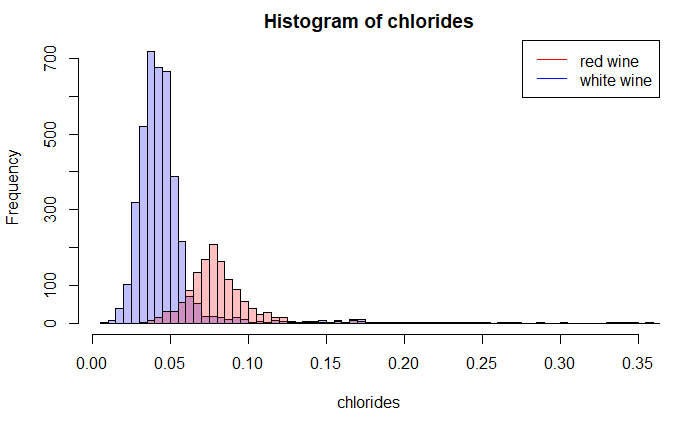
\includegraphics[scale=0.35]{histogram_of_chlorides}
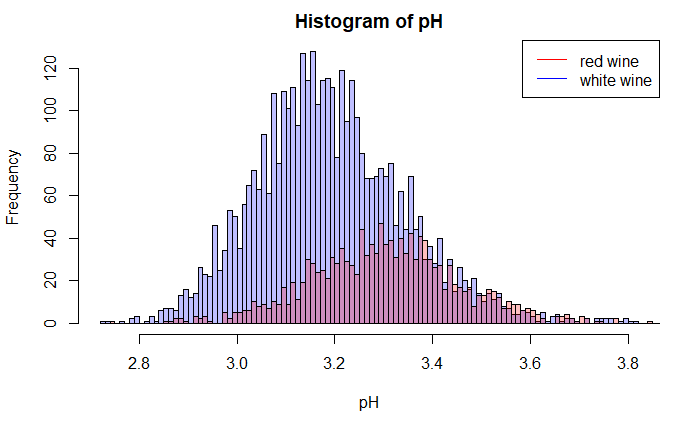
\includegraphics[scale=0.35]{histogram_of_pH}
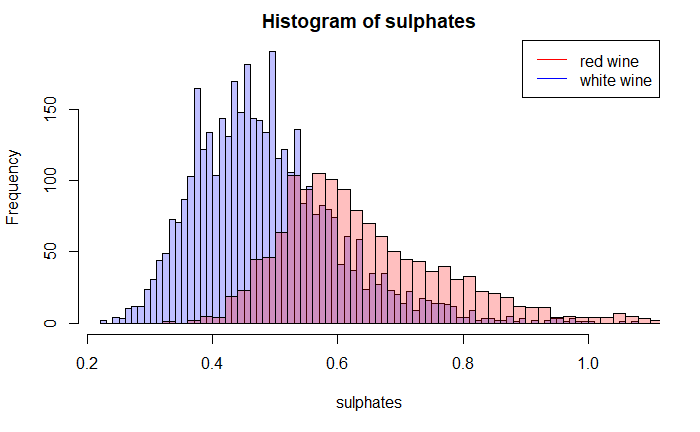
\includegraphics[scale=0.35]{histogram_of_sulphates}
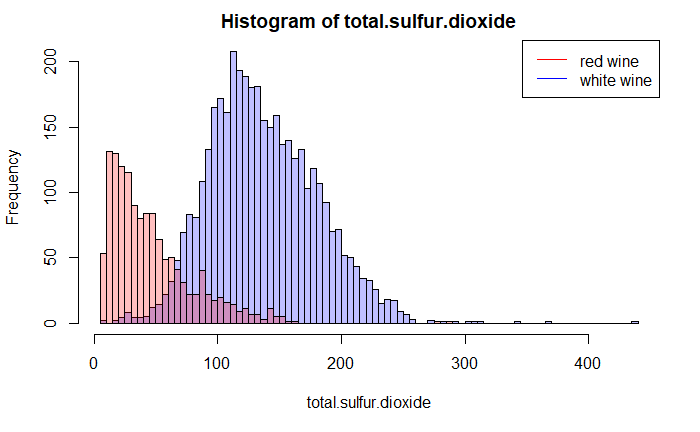
\includegraphics[scale=0.35]{histogram_of_totalsulfurdioxide}
\end{figure}
The next thing we considered was performing a \textbf{PCA}, because it can help us visualize the data and start seeing which variables are more relevant to our goal. We made the following \textit{biplot}, where the first two components explain 50\% of the variability.
\begin{figure}[H]
\centering
\caption{PCA biplot}
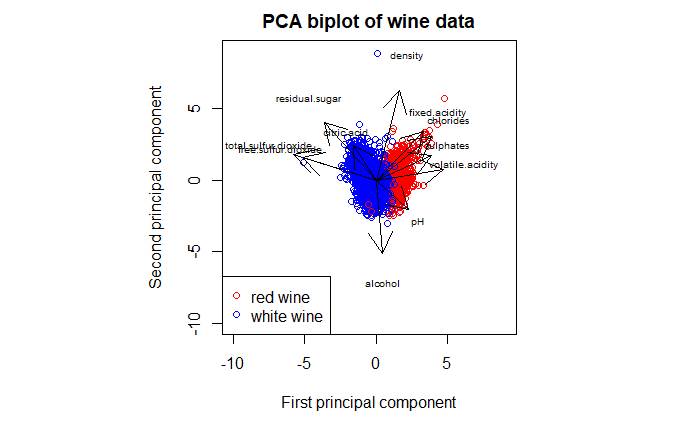
\includegraphics[scale=0.75]{PCA_biplot}
\end{figure}
As the two groups seem to be separated in the horizontal edge, it seems that the \textbf{density and alcohol variables explain very little about the difference between the groups}. However, variables such as \textit{total.sulfur.dioxide} or \textit{volatile.acidity} do. In the PCA we can also see that \textbf{some variables are correlated}, for example, \textit{total.sulfur.dioxide} and \textit{free.sulfur.dioxide} in positive or \textit{density} and \textit{alcohol} in negative. There is a last thing to observe here, the \textbf{outliers}. There are points that are not only far from the others on one variable, but they are so in multiple of them. We will consider whether to remove them or not.   \\

The next thing we can do is a \textbf{bivariate analysis}. We have already seen that some variables may have correlation among them, thus, it is interesting to do the \textit{correlation matrix}. The following graphic is a representation of it using colored circles. \\
\begin{figure}[H]
\centering
\caption{Correlation matrix}
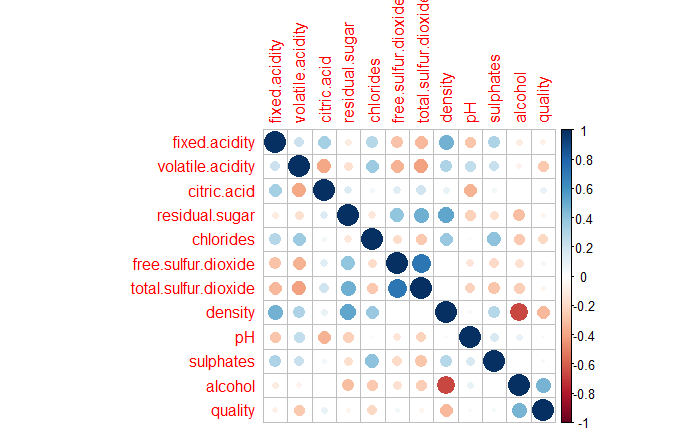
\includegraphics[scale=0.5]{matrix_correlation_circles}
\end{figure}
We have added the \textit{quality} variable, as it can help us have an intuition about which input variables could be useful to predict it. As it can be seen, only few of them have a linear correlation with the target variable. Other variables present mutual correlation, as we suspected.

\section{Resampling protocol \& Modeling methods considered.}
We have separated our data in the following way: we have a \textbf{training set} which has $\frac{2}{3}$ of randomly chosen samples from the whole data set. We will use this training set for model selection. The remaining $\frac13$ of the data goes to the \textbf{testing set}, which we will not use until we want to assess our selected models' performance on new data.\\

As we have a large dataset, we can allow ourselves to be computer-friendly and use \textbf{$K$-fold Cross-Validation} to perform model selection on the training set (we will use $K=10$ throughout all of the work). So, as usual, this involves separating the data into $K$ different subsamples and perform $K$ experiments with each model, fitting it to $K-1$ folds and calculating its \textbf{validation error} when predicting for the held-out fold. Then, these $K$ errors will be averaged and we will have a pretty robust estimation for the error of the model, the \textbf{cross-validation (CV) error}. Out of all the models we train, we will select the ones with less CV-error, and assess them based on their prediction error on new data.\\

As well as we have two problems, we will consider two separate approaches:
\begin{itemize}
	\item To predict the type (red or white), we first considered to apply discriminant methods such as \textbf{LDA}, \textbf{QDA} and \textbf{RDA}, as this is a binary classification problem. Also, we considered to apply \textbf{kNN} (with original, scaled and LD-projected data), and \textbf{Logistic Regression}. We also consider using a \textbf{MLP} and finally also a \textbf{Random Forest} model.
	\item To predict the quality (0 to 10), we have two different approaches:
	\begin{itemize}
		\item The first one, to perform multi-class classification. This can be done via \textbf{LDA}/\textbf{QDA}/\textbf{RDA} as in the type classification, using \textbf{kNN} or using \textbf{Ordinal Regression}.
		\item The second one would be to perform regression and then round the results to obtain a prediction. This first approach could be done with \textbf{Linear Regression} (regularized with both the LASSO $L^1$ and the Ridge $L^2$ methods), \textbf{MLP} and \textbf{RBF-NN} (with just one neuron in the output layer), and \textbf{Random Forest} with regression trees.
	\end{itemize}		
\end{itemize}

\section{Obtained results.}

We have used the original data set without any extracted variables, unless explicitly said so in some sections. We essentially separated our models problem-wise, meaning we have some models for wine type classification and some others for wine quality, for both regression and classification. First of all, we will explain the results for type classification:
\subsection{Wine type prediction}

This problem is modeled as a binary classification. In order to classify the observations, we have used the following methods:
\paragraph{Discriminant Analysis:}
We first of all consider Regularized Discriminant Analysis, as it is the most general method and may help discard LDA or QDA. Applying it, we reached the conclusion that we should directly use LDA, because RDA regularization parameters are $\lambda=1$ and $\gamma$ very close to zero. Now on to LDA. Using $K$-fold CV, with 13 misclassified observations, we reach a cross-validation error of around 0.37\%.

\begin{table}[H]
\centering
\caption{Confusion matrix of LDA}
\begin{tabular}{ccc}
 & Pred as White & Pred as Red \\
Real White & 889 & 6 \\
Real Red  & 7 & 2642
\end{tabular}
\end{table}

\paragraph{$k$ Nearest Neighbors:}
Now, on to kNN; as we know that kNN is very sensitive to the scale of the data, we considered three ways to apply this method. The first one, to use the training set with its original scale. The second one, to use scale dataset. And the third one, to use data projected on to LD space. To see if these changes in the dataset affect the predictions, we considered appropriate to plot the LOOCV error with respect to the first few values of $k$. 
\begin{figure}[H]
\centering
\caption{kNN LOOCV error}
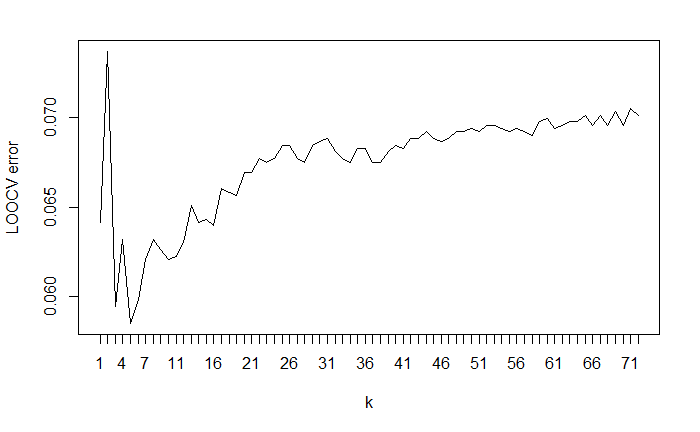
\includegraphics[scale=0.5]{kNN_LOOCV_error}
\end{figure}
In this first approach, we see that the LOOCV decrease quickly and then increases slowly. The minimum error is at $k=5$, with a LOOCV error of roughly 5.8\%. If we scale the data, we can see a clear improvement:
\begin{figure}[H]
\centering
\caption{kNN LOOCV error using scaled data}
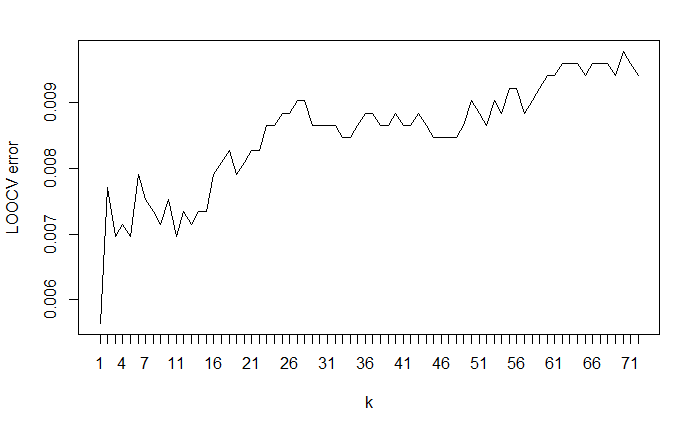
\includegraphics[scale=0.5]{kNN_scaled_LOOCV_error}
\end{figure}
Now the plot presents a minimum at $k=3$ with a LOOCV error of around 0.59\%, so a major improvement have been made. We went further and used kNN with data projected onto LDA space, and the LOOCV error results were the following:
\begin{figure}[H]
\centering
\caption{kNN LOOCV error using LDA projected data}
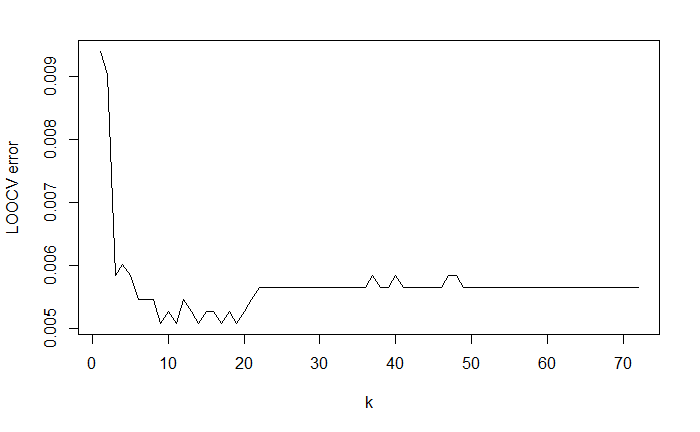
\includegraphics[scale=0.5]{kNN_LDA_LOOCV_error}
\end{figure}
Now the plot is more constant to small values, in particular, the minimum is at $k=8$, with a LOOCV error of 0.34\%. So, for the minimum LOOCV error up until now, we would use this method. Now, we proceed to calculate the cross-validation error from 1 to 25 neighbors. There are several minimums, but the first of them is at $k=5$. As we want to have the simplest model, we will use these value instead of any of the larger ones. This error evaluates to around 0.34\% (12 misclassified). The confusion matrix is the following:\\

\begin{table}[H]
\centering
\caption{Confusion matrix of kNN}
\begin{tabular}{ccc}
 & Pred as White & Pred as Red \\
Real White & 890 & 5 \\
Real Red  & 7 & 2642
\end{tabular}
\end{table}

\paragraph{Logistic Regression:} 
Now we considered a logistic regression model, so a GLM with binomial distribution and logit link. This model gives probabilities of each class, so we had to add a decision boundary for the predicted probability (0.5). In this case the cross-validation error is 0.42\% (15 misclassified), and the confusion matrix is the following:

\begin{table}[H]
\centering
\caption{Confusion matrix of Logistic Regression}
\begin{tabular}{ccc}
 & Pred as White & Pred as Red \\
Real White & 889 & 6 \\
Real Red  & 9 & 2640
\end{tabular}
\end{table}



\paragraph{Multi-Layer Perceptron:}
In order to adjust a reasonable MLP, we have proceeded by fixing a large number of units in a single hidden layer and using weight decay to regularized the model. We considered a MLP with one hidden layer consisting of 20 fixed neurons and variable weight decay parameter. The best decay parameter was selected by cross-validation, and then we calculated the cross validation error of the MLP using the chosen decay parameter. So the error evaluated to 1.3\% (46 misclassified) and the confusion matrix is:

\begin{table}[H]
\centering
\caption{Confusion matrix of MLP}
\begin{tabular}{ccc}
 & Pred as White & Pred as Red \\
Real White & 870 & 25 \\
Real Red  & 21 & 2628
\end{tabular}
\end{table}

\paragraph{Random Forest:}
Now, we consider a Random Forest model. To adjust the number of decision trees we adjusted models with different values for this parameter and then we selected the one with the least out of bag error. We first iterated through the first ten powers of two, which resulted in 256 trees for the minimum oob error. Then around this value we searched for a better number considering the multiples of ten. The final number of trees is 290. Finally, the cross validation error is 0.45\% (16 misclassified) and the confusion matrix is:

\begin{table}[H]
\centering
\caption{Confusion matrix of MLP}
\begin{tabular}{ccc}
 & Pred as White & Pred as Red \\
Real White & 882 & 13 \\
Real Red  & 3 & 2646
\end{tabular}
\end{table}


\subsection{Wine quality prediction}

\subsubsection{Classification}

In this part, we consider the problem of the determining the quality as a multi-class classification problem. We will see that these methods have pretty bad results: this may be due to the classes (which here are the wine marks) being unbalanced. For this reason this section is quite brief.

\paragraph{Discriminant Analysis:} First of all, we have to note that due to some classes having less observations than variables, we cannot perform QDA. So, we directly jump to RDA, whose regularization parameters point towards using only LDA. Then, we adjust a LDA model with the training set, and its cross-validation error amounts to around 45.91\% (1627 misclassified). The confusion matrix is the following:

\begin{table}[H]
\centering
\caption{Confusion matrix of LDA}
\begin{tabular}{cccccccc}
       & Pred 3 & Pred 4 & Pred 5 & Pred 6 & Pred 7 & Pred 8 & Pred 9 \\
Real 3 & 2 & 0 & 9 & 9 & 1 & 0 & 0 \\
Real 4 & 3 & 1 & 76 & 46 & 3 & 0 & 0 \\
Real 5 & 2 & 2 & 674 & 467 & 10 & 0 & 1\\
Real 6 & 1 & 1 & 354 & 1086 & 136 & 0 & 1\\
Real 7 & 0 & 0 & 21 & 378 & 154 & 0 & 0\\
Real 8 & 0 & 0 & 3 & 63 & 36 & 0 & 0\\
Real 9 & 0 & 0 & 0 & 1 & 3 & 0 & 0
\end{tabular}
\end{table}
We can see that this is a pretty bad model, maybe due to the classes being unbalanced as we have said before.

\paragraph{kNN:} So, now on to kNN again. This time, when we check the LOOCV errors to see what is the kNN method (original data, scaled data and LD-projected data) that gives better results, as we did before with the type classification, we see that it is again the one using LD-projected data. So, again our 10-fold cross-validation error function will project the data on to LD space and then perform the kNN classification on this data. Also, we have chosen the $k$ as before, but the minimum is now around $k=55$. To choose the appropriate $k$, we loop over the interval $[50,59]$ and choose the $k$ with the least cross-validation error; we bound the interval with 59 as it is approximately the square root of the number of rows in the training set, and this is a well-known boundary for the number of neighbors.




\subsubsection{Regression}

To predict the wine quality, as expressed above, we used the mwthods of \textbf{LDA}, \textbf{QDA}, \textbf{RDA}, and used the \textbf{kNN} algorithm.\\

Using \textbf{Linear Regression}, we got a testing error of 79.7\%.\\

When performing a \textbf{LDA} and classifying according to the most likely class an accuracy of 0.5496614 was obtained, while for \textbf{QDA} some of the groups were to small in order to be able to perform the analysis accurately, given that the covariance matrix is to be estimated. For instance, the number of wines with a score of 9 was less than the total number of categories, and so this analysis could not be performed with the entirety of the data.\\

For the \textbf{kNN} algorithm, given that the colour variable is a factor type variable, it cannot be directly included to perform the algorithm, as such, two possibilities were considered: that of treating it as a numeric variable equal to 0 or 1 for the two colours, and to disregard the variable completely. In both cases, the algorithm gave similar test accuracies: 0.471219 and 0.46614 respectively when considering the $k=10$ nearest neighbours.\\

Given the distribution of the values in the data set, the algorithm tends to predict mediocre scores for the wines. In other words, given that there were very few outlier wines in the original data set (only five wines had a score of 9) the algorithm cannot predict such a score for wines in the data set. As such, this method is very poor at finding outliers and so it is only partially effective at predicting the score of a wine.
\section{Final Model \& Estimated generalization error.}
\subsection{Wine type best model}
Regarding all the models we have considered, the decision of which we have to select is quite straight-forward as there is a model with the smallest error. We have to note that all the models have a pretty small cross-validation error, being the MLP the greatest. It is very likely that this last model overfits the data. This is a summary of all the models we have considered alongside with their respective errors:

\begin{table}[H]
\centering
\caption{Summary of the models and errors}
\begin{tabular}{ccc}
\textbf{Model} & \textbf{Num. Misclassified} & \textbf{\% Misclassified} \\
LDA & 13 & 0.37 \% \\
kNN & 12 & 0.34 \% \\
Logistic Regression & 15 & 0.42 \% \\
MLP & 46 & 1.3 \% \\
Random Forest & 16 & 0.45 \%
\end{tabular}
\end{table}

Clearly, the least error belongs to the kNN model using the LD projected data and $k=5$. Finally, the testing error is 0.96\% (17 misclassified) and the confusion matrix is:

\begin{table}[H]
\centering
\caption{Confusion matrix of kNN}
\begin{tabular}{ccc}
 & Pred as White & Pred as Red \\
Real White & 454 & 8 \\
Real Red  & 9 & 1301
\end{tabular}
\end{table}



\subsection{ best model}

\section{Scientific and personal conclusions.}
\section{Possible extensions and known limitations.}
%\section{Future approaches.}
%To accomplish a \textbf{good and simple method}, we will continue trying the methods we already mention. Reducing the number of input variables, adding some extracted variables or with small variations of the methods (like applying \textit{pca} or \textit{lda} before \textit{glm} or \textbf{ridge regression}). In addition, we will consider other methods for classification as well for data exploration. For example, using \textbf{Random Forest}, \textbf{neural networks} or \textbf{clustering}.
\section{References:}
\begin{enumerate}
  \item Web page where the data set can be found:

  \href{http://archive.ics.uci.edu/ml/datasets/Wine+Quality}{ http://archive.ics.uci.edu/ml/datasets/Wine+Quality}

  \item Relevant paper (a previous approach):

  \href{https://www.sciencedirect.com/science/article/pii/S0167923609001377?via\%3Dihub}{ https://www.sciencedirect.com/science/article/pii/S0167923609001377?via\%3Dihub}

  \item Kernels that study this data set on Kaggle (\href{www.kaggle.com}{kaggle.com}):

  \href{https://www.kaggle.com/indra90/predicting-white-wine-quality}{First kernel: https://www.kaggle.com/indra90/predicting-white-wine-quality},\\
  \href{https://www.kaggle.com/conradws/how-good-is-this-wine-m-l-for-quality-control}{Second kernel: https://www.kaggle.com/conradws/how-good-is-this-wine-m-l-for-quality-control},\\
  \href{https://www.kaggle.com/danielpanizzo/red-and-white-wine-quality}{Third kernel: https://www.kaggle.com/danielpanizzo/red-and-white-wine-quality}.

  \item Exploratory Data Analysis notebooks:

  \href{https://rstudio-pubs-static.s3.amazonaws.com/57835\_c4ace81da9dc45438ad0c286bcbb4224.html}{ https://rstudio-pubs-static.s3.amazonaws.com/57835\_c4ace81da9dc45438ad0c286bcbb4224.html},\\
  \href{https://rstudio-pubs-static.s3.amazonaws.com/219996\_9cc8cf9f2e7e41fe8912454c3ad2685a.html}{ https://rstudio-pubs-static.s3.amazonaws.com/219996\_9cc8cf9f2e7e41fe8912454c3ad2685a.html}.



\end{enumerate}



\end{document} 